\documentclass[a4paper]{article}
\usepackage[utf8]{inputenc}
\usepackage{amsmath}
\usepackage{polski}
\usepackage[polish]{babel}
\usepackage[T1]{fontenc}
\usepackage[a4paper,top=3cm,bottom=2cm,left=3cm,right=3cm,marginparwidth=1.75cm]{geometry}
\usepackage{graphicx}
\usepackage{float}
\usepackage{longtable}
\usepackage{pdflscape}
\usepackage[backend=bibtex]{biblatex}
\graphicspath{{../img/}}

\title{Optymalizacja fabryki z wykorzystaniem algorytmu immunologicznego (selekcji klonalnej)}
\author{Artur Bauer \and Kamil Szostek \and Sławomir Goździewski \and Wiktor Filipiak}
\date{\today}

\usepackage[pdftex,
            pdfauthor={Artur Bauer \& Kamil Szostek \& Sławomir Goździewski \& Wiktor Filipiak},
            pdftitle={\@title},
            pdfsubject={Glebokie uczenie i inteligencja obliczeniowa},
            pdfkeywords={Automatyka i Robotyka},
            pdfproducer={Latex},
            pdfcreator={pdflatex}]{hyperref}

\bibliography{citations.bib}

\begin{document}
%--------------------------------------------------------%
%	COVER PAGE
%--------------------------------------------------------%

\begin{titlepage}
\makeatletter

  \newcommand{\HRule}{\rule{\linewidth}{0.5mm}} % Defines a new command for the horizontal lines, change thickness here

  \center % Center everything on the page


%	HEADING SECTION

  \textsc{\LARGE Akademia Górniczo-Hutnicza}\\[1.5cm] % Name of your university/college
  \textsc{\Large  Głębokie uczenie i inteligencja obliczeniowa }\\[0.5cm] % Major heading such as course name
  \textsc{\large Automatyka i Robotyka II Stopień}\\[0.5cm] % Minor heading such as course title
  \textsc{2019/2020}\\[0.5cm] % Minor heading such as course title

%	TITLE SECTION

  \vspace{1.5 cm}
  \HRule \\[0.4cm]
  { \huge \bfseries \@title} \\[0.4cm] % Title of your document
  \HRule \\[1.5cm]
 
%	AUTHOR SECTION

  {\em\Large\textbf Skład zespołu:}\\
  \vspace{.5 cm}
    Artur Bauer\\
    Kamil Szostek\\
    Sławomir Goździewski\\
    Wiktor Filipiak
  \vspace{1.5 cm}
  
  
  {\em\Large\textbf Opiekun:}\\
  \vspace{.5 cm}
  dr hab. inż. Joanna Kwiecień
  
%	DATE SECTION

  \vspace{1.5 cm}
  {\large Złożono: \@date}\\[3cm] % Date, change the \today to a set date if you want to be precise


\vfill % Fill the rest of the page with whitespace

\end{titlepage}

%-----------------------------------------------------------------

\newpage

\tableofcontents

\newpage
\section{Wstęp}
\subsection{Factory model}\label{factory}

\begin{figure}[ht]
\centering
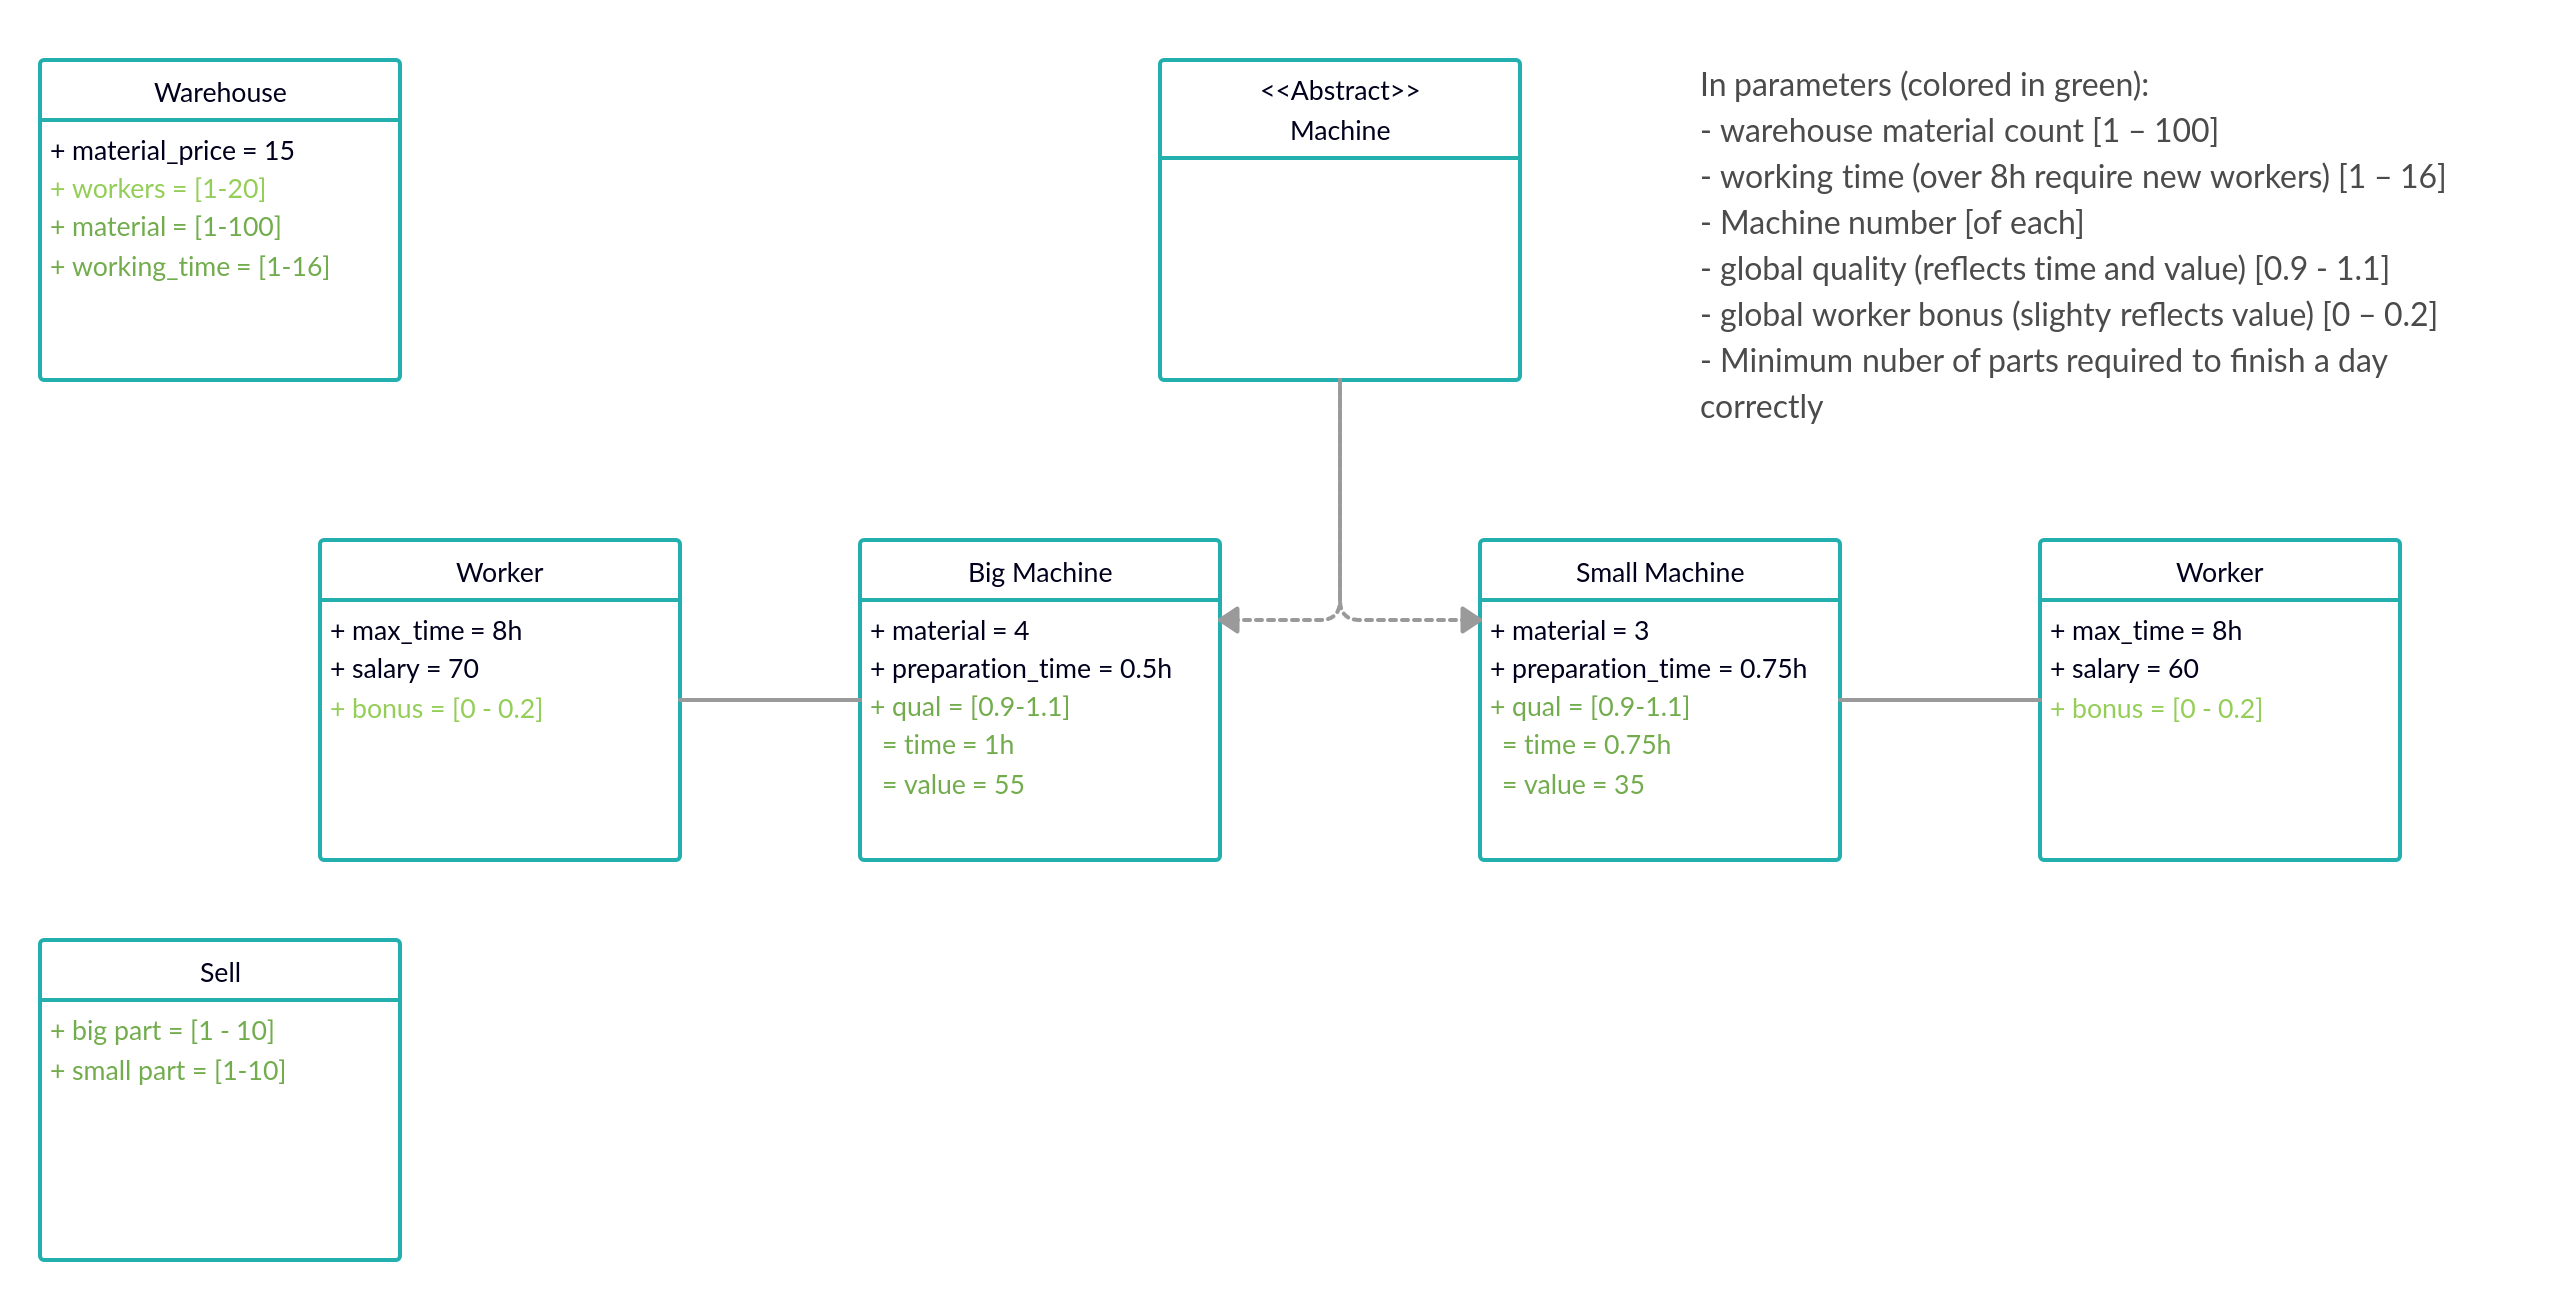
\includegraphics[width=.7\textwidth]{Factory_scheme.png}
\caption{Model fabryki}
\end{figure}

\subsubsection{Funkcja celu fabryki:}

$$Income = \sum^{n_p}_{i=1}(p_i*(v_i-m_i*m_p)) - (1+b_i)*\sum^{n_w}_{i = 1}(w_i*s_i *t_{wi}) - m_r*m_p - punish$$

Gdzie:
\begin{itemize}
    \item $n_p$ -- ilość rodzajów części
    \item $p_i (n_m)$ -- ilość wyprodukowanych części i-tego typu
    \item $v_i(v_{bi}, t_{wi},t_{bi},w_q)$ -- wartość części i-tego typu
    \item $m_i$ -- liczba surowca potrzebna do wytworzenia elementu i-tego typu
    \item $m_p$ -- cena surowca
    \item $n_w$ -- liczba rodzajów pracowników
    \item $w_i$ -- liczba pracowników i-tego rodzaju
    \item $s_i$ -- wypłata pracownika i-tego rodzaju
    \item $b$ -- premia pracownicza
    \item $m_r(p_i,n_m)$ -- pozostały materiał
    \item $p_{i_{min}}$ -- minimalna ilość elementów do wytworzenia i uniknięcia kary
    \item $p_{i_{max}}$ -- maksymalna ilość wytworzonych elementów
    \item $n_m$ -- liczba surowca na początek dnia
\end{itemize}
\subsubsection{Kara}
$punish = p_{un}*\sum^{n_p}_{i=1}(p_{num_i})*v_i$

$p_{num_i}= \left\{\begin{matrix} 0  \;\quad\quad\quad\quad  \textrm{if} \quad  p_{i_{min}}-p_i \leq  0    \\ p_{i_{min}}-p_i  \quad  \textrm{if} \quad  p_{i_{min}}-p_i >  0  \end{matrix}\right.$

Where: 
\begin{itemize}
    \item $p_{un}$ -- współczynnik kary
    \item $p_{num_i}(p_{i_{min}}, p_i)$ -- liczba elementów i-tego typu dla których naliczana jest kara
\end{itemize}
\subsubsection{Liczba pracowników}

Liczba pracowników i-tego typu jest równa ilości maszyn i-tego typu:

$n_p = n_w$

\subsubsection{Maksymalna ilość elementów}\label{max-number-of-items}

Niezbędna ilość elementów i-tego typu:

$\sum^{n_p}_{i=1} p_{i_{max}} * m_i< n_m$

\subsubsection{Rzeczywisty czas pracy maszyny na 1 produkt}\label{real-working-time-of-the-i-type-machineemployee-for-one-product} $t_{wi} = t_{pi} + p_i * t_{bi}$

\subsection{Parametry modelu}\label{model-assumption}

\begin{longtable}[c]{lll}
Parametr & oznaczenie & wartość\\ \hline
Ilość surowców & $n_m$ & [$x$ - 100]\\
Koszt surowca & $m_p$ & 15\\
Czas pracy & ? & {[}1 - 16{]}\\
Minimalna ilość dużych części & $p_{0_{min}}$ & [0 - 10]\\
Minimalna ilość małych części & $p_{1_{min}}$ & [0 -10]\\
Wypłata operatora dużej maszyny & $s_0$ & 70\\
Wymagana ilość materiału na duży element & $m_0$ & 4\\
Czas przygotowania dużej maszyny & $t_{p0}$ & 30 min\\
Wartość dużego elementu & $v_{b0}$ & 50\\
Podstawowy czas pracy na duży element & $t_{b0}$ & 1h\\
Liczba dużych maszyn & ? & [0 - 10]\\
Wypłata operatora małej maszyny & $s_1$ & 60\\
Ilość surowca na mały element & $m_1$ & 3\\
Czas przygotowania małej maszyny & $t_{p1}$ & 45 min\\
Wartość małego elementu & $v_{b1}$ & 35\\
Czas wytworzenia małego elementu & $t_{b1}$ & 45 min\\
Ilość małych maszyn & ? & [0 - 10]\\
Maksymalny czas pracy pracownika & ? & 8h\\
Bonus pracowniczy & b & [0.0 - 0.2]\\
Współczynnik kary & $p_{un}$ & 1.5
\end{longtable}

Gdzie:
\begin{itemize}
    \item $x$ -- ilość wymaganych elementów * koszt części 
    \item Parametry wejściowe podane są w kwadratowych nawiasach
    \item Pracownik jest zatrudniony na pełen etat (8h płacone z góry)
    \item Pierwsza i druga zmiana są identyczne w ilość i rodzaj maszyn i pracowników
    \item Rezerwujemy surowce na wymagane elementy
    \item Wszystkie elementy ponad wymaganą liczbę są eksta dochodem
\end{itemize}


\section{Badany problem}
\subsection{Przegląd literatury}
This article is about the Clonal Selection Algorithm used for Optimalization in Electromagnetics. The authors present their own concept of real-coded clonal selection algorithm that can be used in electromagnetic design optimization. The article describes in detail all the algorithm parameters as well as the operation of the algorithm for "The TEAM Workshop problem 22”\cite{1430953}.



This article is about the artificial immune system in industrial application. Basing on cutting parameters (force, vibrations, torque etc.) they try to detect tool brake using a negative-selection algorithm \cite{dasgupta1999artificial}.



This article is about the artificial immune system in industrial application. Authors compare AIS with Social Learning Mechanisms to few others AIS which use cloning alghoritm. Basing on proportional–/integral–/derivative-time they try to tune a PID \cite{wang_artificial_2017}.



This article is about the Clonal Selection Based Memetic Algorithm for Job Shop Scheduling Problems. The authors' goal was to improve exploration and exploitation using a clonal selection algorithm. The article presents the use of clonal selection to construct an evolutionary search mechanism that is used for exploration\cite{yang2008clonal}.


This article is about Clonal Selection Algorithm in engineering applications. It describes theoretical functioning of the algorithm and illustrates the workings of implemented algorithm on three different problems: a binary character recognition, multi-modal optimization of function – 
$f(x, y) = x.\sin(4 \pi x) - y.\sin(4 \pi y + \pi) + 1$
and Traveling Salesman Problem for 30 cities \cite{de_castro}.


This article is about using Clonal Selection Algorithm to optimize the layout of a construction site. Presented algorithm is used to minimize production costs and traveling distance between n facilities which are represented in n x n permutation matrix \cite{WANG2016267}.


This article is about the Artificial Immune System for solving the Capacitated Vehicle Routing Problem. The objective of the article was to investigate the suitable setting of clonal selection AIS parameters for solving the CVRP through the statistical design of experiment. The article also shows the performance of AIS and other methods for benchmarking twenty CVRP instances in terms of the quality of solutions and the computational time used \cite{thapatsuwan}.


This article is about using Clonal Selection Algorithm in determining optimal operation points in hybrid AC/DC low voltage microgrid. The objective was to minimize active power losses, operation costs and optimize nodal voltage level \cite{rokicki}.



\section{Diagram UML fabryki}
\begin{figure}[ht]
\centering
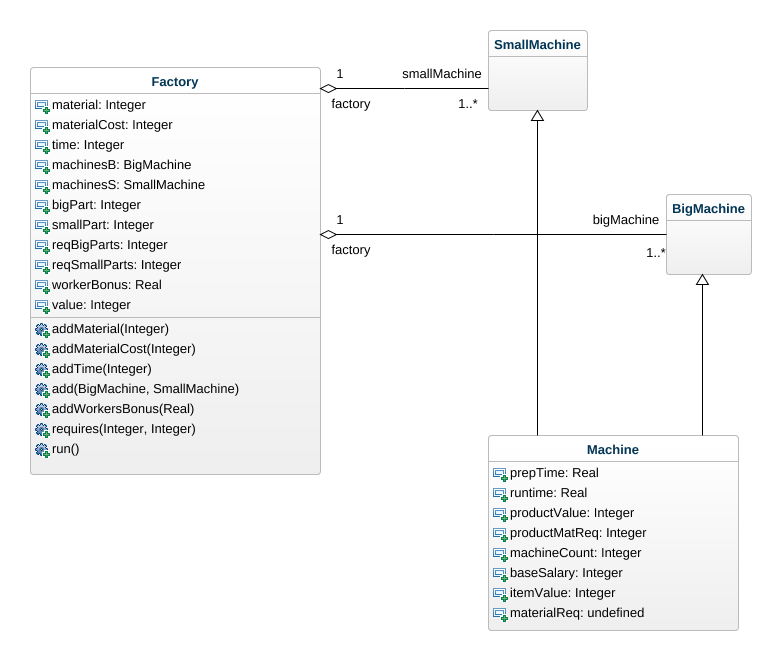
\includegraphics[width=.7\textwidth]{UML_Model.png}
\caption{Diagram UML}
\end{figure}

\newpage
\printbibliography

\end{document}

